\chapter{Results}
\label{chap:Results}

The observed number of events in the various control regions are
included in a fit that uses the profile likelihood ratio method to determine the SM background
estimates in each signal region. This procedure takes common
systematic uncertainties (discussed in Section~\ref{sec:Systematics}) between the
control and signal regions and their correlations into account; they are treated as nuisance
parameters in the fit and are modelled by Gaussian probability density
functions.

In general control regions are designed for as many of the SRs as possible. However, due to statistical limitation three CRs are used for all SRs: CRW, CRST, CRTTGamma. For these regions a choice needs to be made for which of the specially designed CRTop and CRZ regions should be used in the fits. Below is a summary:
\begin{itemize}
  \item CRW: Due to the top mass veto the only CRs without an ISR or top mass requirement are used in CRW. These are CRZD and CRTopD. 
  \item CRST: it was found that this CR was mainly populated with events that fall in the T0 category (66\%). For this reason, CRZAB-T0 is used for the Z fit. The \met\ requirements of CRTopB are closer to CRST and thus CRTopB is used for the top background fit. 
  \item \ttbar+V: For CRTop, CRTopBT0 was chosen again because the T0 made up a large part of the events (40\%) in CRTTGamma.
For similar reasons, CRZAB-T0 is used for the Z background.
\end{itemize}

Three different likelihood fits are performed to extract the results. \\
{\bf Background-only fit}: Only the control regions are used to constrain
the fit parameters. Potential signal contamination is neglected and
the number of observed events in the signal regions is not taken into
account in the fit. \\
{\bf Exclusion fit:} Both control and signal regions are used to
constrain the fit parameters. The signal contribution as predicted by
the tested model is taken into account in both regions using an
additional free parameter for the non-SM signal strength in the
likelihood fit that is constrained to be non-negative. Since the
observed event yield in the signal region is used, the background
prediction can differ from the prediction on the background-only fit. The exclusion fit configuration is used to produce all the model-dependent limits.\\
{\bf Discovery fit:} Both control and signal regions are used to constrain the fit parameters. A potential signal contribution is considered in the signal regions but neglected in the control regions. This background prediction is conservative since any signal contribution in the control regions is attributed to background and thus yields a possible overestimate of the background in the signal regions. The discovery fit configuration is used to produce upper limits on the visible cross-sections.

% The fit configuration is described in Section~\ref{sec:StatAnalysis} 
The \verb+HistFitter+
results with data samples are
described in
Section~\ref{sec:bkgOnlyFit}. 

\clearpage



\subsection{Unblinded distributions}
\label{sec:unblindedDists}

Figures~\ref{fig:SRAUnblined},~\ref{fig:SRBUnblined},~\ref{fig:SRCUnblined},~\ref{fig:SRDUnblined},~\ref{fig:SREUnblined} show the postfit, unblinded distribution of some of the most discriminating variables of SRA, SRB, SRC, SRD, and SRE at \intlumi\ \ifb. For SRA and SRB the distributions for individual categories are shown. Additionally, the error bands include both MC statistical and all detector systematical uncertainties. 


\begin{figure}[!hp] 
\begin{center}
%\includegraphics[width=0.45\textwidth]{figures/SRC/CA_RISR_SRC}
\caption{Unblinded \rISR\ and \pTISR\ distributions for SRC1-5 for \intlumi\ \ifb.}
\label{fig:SRCUnblined}
\end{center}
\end{figure}








%%%%%
%comment out ichep results starts here @@

\clearpage
\subsection{Background-only fit}
\label{sec:bkgOnlyFit}
The background-only fit 
has been performed taking the dominant experimental systematics and
the theoretical systematics for $W/Z$+jets and \ttbar~(RadLoHi and PowhegHerwigpp only) 
into account ({\bf to be updated}).
The yields in the control regions, normalized to \intlumi\ \ifb are shown
in Tables \ref{table.bkgonly.CRTopA}, \ref{table.bkgonly.CRTopB},
\ref{table.bkgonly.CRTopCDE}, \ref{table.bkgonly.CRTTgamma},
\ref{table.bkgonly.CRZ} and \ref{table.bkgonly.CRother}. 
The resulting scale factors for the backgrounds are summarized in Table
\ref{table.scale.factors}. The yields in the validation regions
are shown in Tables \ref{table.bkgonly.VRTopA},
\ref{table.bkgonly.VRTopB}, \ref{table.bkgonly.VRTop},
\ref{table.bkgonly.VRW}
and \ref{table.bkgonly.VRZ}.
The background yields in the signal regions, normalized to
\intlumi\ \ifb, are shown in Tables
\ref{table.bkgonly.SRA},\ref{table.bkgonly.SRB},\ref{table.bkgonly.SRC1to3},\ref{table.bkgonly.SRC4to5},\ref{table.bkgonly.SRD},and
\ref{table.bkgonly.SRE}; the signal regions are now unblinded and the
number of events seen in the data are also shown.

The
breakdown of the post-fit systematic uncertainties, summed over the
backgrounds, is shown in Tables
\ref{table.results.bkgestimate.uncertainties.SRA_TT_SRA_TW_SRA_T0},
\ref{table.results.bkgestimate.uncertainties.SRB_TT_SRB_TW_SRB_T0},
\ref{table.results.bkgestimate.uncertainties.SRC1_SRC2_SRC3},
\ref{table.results.bkgestimate.uncertainties.SRC4_SRC5},
\ref{table.results.bkgestimate.uncertainties.SRD_low_SRD_high} and
\ref{table.results.bkgestimate.uncertainties.SRE}.
The breakdown of the post-fit systematic uncertainties, summed over
the backgrounds, but separated by signal region (so that the ordering
is clearer in each signal region) can be found in Appendix
\ref{sec:bkgonly_fit_details}. 
% An
% even-more detailed breakdown of the systematic uncertainties,
% separated by background source, can be found in Appendix
% \ref{sec:HistFitter.20.7}.  The breakdown of pre-fit systematic
% uncertainties for benchmark signal samples can also be found in the Appendix.

A plot of the correlation between fit parameters of interest and the
nuisance parameters is shown in Fig. \ref{figure.corrMatrix} and the
post-fit pull plot for the background-only fit is shown in
Fig. \ref{figure.pullPlot}.
% while Table~\ref{table.pulls}
% shows the post-fit pulls for the exclusion fit for T800\_L1 for
% SRA. The pull table shows that there is no profiling or pulling of the
% nuisance parameters.

% A selection of post-fit plots in validation and signal regions,
% following the background-only fit can be found in Appendix
% \ref{sec:afterFitPlots.20.7}.

\begin{table}
  \begin{center}
    \begin{tabular*}{\textwidth}{@{\extracolsep{\fill}}lr}
      \noalign{\smallskip}\hline\noalign{\smallskip}
      {\bf MC sample}           & Fitted scale factor        \\[-0.05cm] \hline
      ttbar &   $0.707 \pm 0.050$             \\
      W+jets &   $1.27 \pm 0.15$              \\
      Single top &   $1.17 \pm 0.39$              \\
      ttbar$\gamma$ &   $1.29 \pm 0.20$              \\ \hline
    \end{tabular*}

  \end{center}
  \caption{Fitted scale factors for the MC background samples based on
    \intlumi\ \ifb of data.}
  \label{table.scale.factors}
\end{table}



\begin{table}
\begin{center}
\setlength{\tabcolsep}{0.0pc}
{\small
%%
\begin{tabular*}{\textwidth}{@{\extracolsep{\fill}}lrrr}
\noalign{\smallskip}\hline\noalign{\smallskip}
{\bf CRTopCDE yields}           & CRTopC            & CRTopD            & CRTopE              \\[-0.05cm]
\noalign{\smallskip}\hline\noalign{\smallskip}
%%
Observed events          & $611$              & $157$              & $50$                    \\
\noalign{\smallskip}\hline\noalign{\smallskip}
%%
Fitted bkg events         & $610.96 \pm 24.72$          & $156.89 \pm 12.52$          & $49.99 \pm 7.07$              \\
\noalign{\smallskip}\hline\noalign{\smallskip}
%%
        Fitted TTbar events         & $461.47 \pm 31.85$          & $130.35 \pm 13.67$          & $42.94 \pm 7.27$              \\
%%
        Fitted Wjets events         & $64.94 \pm 12.12$          & $5.13 \pm 1.05$          & $2.17 \pm 0.36$              \\
%%
        Fitted Zjets events         & $2.15 \pm 0.90$          & $0.09 \pm 0.06$          & $0.02 \pm 0.01$              \\
%%
        Fitted TtbarV events         & $11.32 \pm 2.19$          & $2.85 \pm 0.70$          & $1.08 \pm 0.42$              \\
%%
        Fitted SingleTop events         & $63.49 \pm 20.36$          & $17.14 \pm 5.88$          & $2.31 \pm 0.78$              \\
%%
        Fitted Diboson events         & $7.58 \pm 2.84$          & $1.33_{-1.33}^{+1.75}$          & $1.47_{-1.47}^{+1.74}$              \\
%%
        Fitted Multijets events         & $0.00 \pm 0.00$          & $0.00 \pm 0.00$          & $0.00 \pm 0.00$              \\
%%     
 \noalign{\smallskip}\hline\noalign{\smallskip}
%%
MC exp. SM events              & $777.01 \pm 14.91$          & $160.22 \pm 5.32$          & $48.46 \pm 2.87$              \\
\noalign{\smallskip}\hline\noalign{\smallskip}
%%
        MC exp. TTbar events         & $652.93 \pm 7.35$          & $137.86 \pm 3.58$          & $42.45 \pm 2.04$              \\
%%
        MC exp. Wjets events         & $51.34 \pm 6.02$          & $4.05 \pm 0.50$          & $1.71 \pm 0.16$              \\
%%
        MC exp. Zjets events         & $1.84 \pm 0.58$          & $0.09 \pm 0.06$          & $0.02 \pm 0.01$              \\
%%
        MC exp. TtbarV events         & $8.78 \pm 0.90$          & $2.21 \pm 0.38$          & $0.84 \pm 0.29$              \\
%%
        MC exp. SingleTop events         & $54.53 \pm 5.03$          & $14.70 \pm 2.08$          & $1.98 \pm 0.17$              \\
%%
        MC exp. Diboson events         & $7.58 \pm 2.87$          & $1.32_{-1.32}^{+1.74}$          & $1.46_{-1.46}^{+1.74}$              \\
%%
        MC exp. Multijets events         & $0.00 \pm 0.00$          & $0.00 \pm 0.00$          & $0.00 \pm 0.00$              \\
%%     \\
\noalign{\smallskip}\hline\noalign{\smallskip}
\end{tabular*}
%%%
}
\end{center}
\caption{Region: CRTopCDE. Background-only fit results for an integrated luminosity of 36.07 \ifb. The uncertainties are statistical and systematic.
}
\label{table.bkgonly.CRTopCDE}
\end{table}
%



\begin{table}
\begin{center}
\setlength{\tabcolsep}{0.0pc}
{\small
%%
\begin{tabular*}{\textwidth}{@{\extracolsep{\fill}}lrrr}
\noalign{\smallskip}\hline\noalign{\smallskip}
{\bf VRTop yields}           & VRTopC            & VRTopD            & VRTopE              \\[-0.05cm]
\noalign{\smallskip}\hline\noalign{\smallskip}
%%
Observed events          & $281$              & $238$              & $106$                    \\
\noalign{\smallskip}\hline\noalign{\smallskip}
%%
Fitted bkg events         & $277.97 \pm 17.53$          & $193.21 \pm 20.29$          & $83.53 \pm 21.79$              \\
\noalign{\smallskip}\hline\noalign{\smallskip}
%%
        Fitted TTbar events         & $156.22 \pm 15.28$          & $164.44 \pm 21.50$          & $69.17 \pm 22.06$              \\
%%
        Fitted Wjets events         & $43.25 \pm 9.44$          & $3.94 \pm 0.91$          & $2.27 \pm 0.77$              \\
%%
        Fitted Zjets events         & $39.09 \pm 9.93$          & $5.89 \pm 1.19$          & $4.43 \pm 1.00$              \\
%%
        Fitted TtbarV events         & $8.89 \pm 1.43$          & $4.72 \pm 0.89$          & $3.08 \pm 0.78$              \\
%%
        Fitted SingleTop events         & $24.92 \pm 8.61$          & $13.34 \pm 4.65$          & $3.76 \pm 1.23$              \\
%%
        Fitted Diboson events         & $5.60 \pm 1.63$          & $0.88 \pm 0.41$          & $0.82 \pm 0.46$              \\
%%     
 \noalign{\smallskip}\hline\noalign{\smallskip}
%%
MC exp. SM events              & $335.59$          & $183.91$          & $78.42$              \\
\noalign{\smallskip}\hline\noalign{\smallskip}
%%
        MC exp. TTbar events         & $231.65$          & $159.35$          & $66.46$              \\
%%
        MC exp. Wjets events         & $38.56$          & $3.51$          & $2.02$              \\
%%
        MC exp. Zjets events         & $32.23$          & $5.45$          & $3.59$              \\
%%
        MC exp. TtbarV events         & $6.97$          & $3.70$          & $2.41$              \\
%%
        MC exp. SingleTop events         & $20.58$          & $11.01$          & $3.11$              \\
%%
        MC exp. Diboson events         & $5.60$          & $0.88$          & $0.82$              \\
%%     \\
\noalign{\smallskip}\hline\noalign{\smallskip}
\end{tabular*}
%%%
}
\end{center}
\caption{Region: VRTopCDE. Background-only fit results for an integrated luminosity of 36.47 \ifb. The uncertainties are statistical and systematic.
}
\label{table.bkgonly.VRTop}
\end{table}
%

\clearpage



\begin{table}
\begin{center}
\setlength{\tabcolsep}{0.0pc}
{\small
%%
\begin{tabular*}{\textwidth}{@{\extracolsep{\fill}}lrrr}
\noalign{\smallskip}\hline\noalign{\smallskip}
{\bf SRC yields}           & SRC1            & SRC2            & SRC3              \\[-0.05cm]
\noalign{\smallskip}\hline\noalign{\smallskip}
%%
Observed events          & $23$              & $22$              & $23$                    \\
\noalign{\smallskip}\hline\noalign{\smallskip}
%%
Fitted bkg events         & $13.89 \pm 2.89$          & $25.32 \pm 4.29$          & $18.02 \pm 2.64$              \\
\noalign{\smallskip}\hline\noalign{\smallskip}
%%
        Fitted TTbar events         & $11.25 \pm 2.99$          & $21.39 \pm 3.67$          & $14.64 \pm 2.36$              \\
%%
        Fitted Wjets events         & $0.64 \pm 0.19$          & $1.59 \pm 0.44$          & $1.54 \pm 0.57$              \\
%%
        Fitted Zjets events         & $0.00 \pm 0.00$          & $0.00 \pm 0.00$          & $0.00 \pm 0.00$              \\
%%
        Fitted TtbarV events         & $0.16_{-0.16}^{+0.28}$          & $0.52 \pm 0.44$          & $0.49 \pm 0.31$              \\
%%
        Fitted SingleTop events         & $1.42 \pm 0.98$          & $1.57 \pm 1.04$          & $0.85 \pm 0.36$              \\
%%
        Fitted Diboson events         & $0.41 \pm 0.24$          & $0.24 \pm 0.05$          & $0.51 \pm 0.20$              \\
%%     
 \noalign{\smallskip}\hline\noalign{\smallskip}
%%
MC exp. SM events              & $18.96$          & $35.08$          & $24.66$              \\
\noalign{\smallskip}\hline\noalign{\smallskip}
%%
        MC exp. TTbar events         & $16.68$          & $31.72$          & $21.70$              \\
%%
        MC exp. Wjets events         & $0.57$          & $1.42$          & $1.37$              \\
%%
        MC exp. Zjets events         & $0.00$          & $0.00$          & $0.00$              \\
%%
        MC exp. TtbarV events         & $0.13$          & $0.41$          & $0.38$              \\
%%
        MC exp. SingleTop events         & $1.17$          & $1.29$          & $0.70$              \\
%%
        MC exp. Diboson events         & $0.41$          & $0.24$          & $0.51$              \\
%%     \\
\noalign{\smallskip}\hline\noalign{\smallskip}
\end{tabular*}
%%%
}
\end{center}
\caption{Region: SRC. Background-only fit results for an integrated luminosity of 36.47 \ifb. The uncertainties are statistical and systematic.
}
\label{table.bkgonly.SRC1to3}
\end{table}
%



\begin{table}
\begin{center}
\setlength{\tabcolsep}{0.0pc}
{\small
%%
\begin{tabular*}{\textwidth}{@{\extracolsep{\fill}}lrr}
\noalign{\smallskip}\hline\noalign{\smallskip}
{\bf SRC yields}           & SRC4            & SRC5              \\[-0.05cm]
\noalign{\smallskip}\hline\noalign{\smallskip}
%%
Observed events          & $1$              & $0$                    \\
\noalign{\smallskip}\hline\noalign{\smallskip}
%%
Expected bkg events         & $8.14 \pm 1.39$          & $0.99 \pm 0.71$              \\
\noalign{\smallskip}\hline\noalign{\smallskip}
%%
        Expected TTbar events         & $4.92 \pm 0.98$          & $0.63_{-0.63}^{+0.69}$              \\
%%
        Expected Wjets events         & $1.93 \pm 0.45$          & $0.21 \pm 0.12$              \\
%%
        Expected Zjets events         & 0.45 $\pm$ 0.24          & 0.09 $\pm$ 0.04             \\
%%
        Expected TtbarV events         & $0.08 \pm 0.08$          & $0.06 \pm 0.03$              \\
%%
        Expected SingleTop events         & $0.72_{-0.72}^{+0.77}$          & $0.00 \pm 0.00$              \\
%%
        Expected Diboson events         & $0.00 \pm 0.00$          & $0.00 \pm 0.00$              \\
%%
        Expected Multijets events         & $0.04 \pm 0.02$          & $0.00 \pm 0.00$              \\
%%     
 \noalign{\smallskip}\hline\noalign{\smallskip}
\end{tabular*}
%%%
}
\end{center}
\caption{Region: SRC. Background-only fit results for an integrated luminosity of 36.07 \ifb. The uncertainties are statistical and systematic.
}
\label{table.bkgonly.SRC4to5}
\end{table}
%


\clearpage


\begin{table}
\begin{center}
\setlength{\tabcolsep}{0.0pc}
\begin{tabular*}{\textwidth}{@{\extracolsep{\fill}}lccc}
\noalign{\smallskip}\hline\noalign{\smallskip}
{\bf Uncertainty of channel}                                    & SRC1            & SRC2            & SRC3            \\
\noalign{\smallskip}\hline\noalign{\smallskip}
%%
Total background expectation             &  $20.56$        &  $27.54$        &  $18.86$       \\
%% \\
\noalign{\smallskip}\hline\noalign{\smallskip}
%%
Total statistical $(\sqrt{N_{\rm exp}})$              & $\pm 4.53$        & $\pm 5.25$        & $\pm 4.34$       \\
%%
Total background systematic               & $\pm 6.62\ [32.18\%] $        & $\pm 4.89\ [17.75\%] $        & $\pm 3.53\ [18.72\%] $             \\
\noalign{\smallskip}\hline\noalign{\smallskip}
\noalign{\smallskip}\hline\noalign{\smallskip}
%%
alpha\_ttbarGenPS         & $\pm 4.86\ [23.6\%] $          & $\pm 1.91\ [6.9\%] $          & $\pm 2.39\ [12.7\%] $       \\
%%
alpha\_RadLoHi         & $\pm 2.64\ [12.8\%] $          & $\pm 2.19\ [8.0\%] $          & $\pm 1.06\ [5.6\%] $       \\
%%
alpha\_JetSmearing         & $\pm 2.38\ [11.6\%] $          & $\pm 0.77\ [2.8\%] $          & $\pm 0.17\ [0.91\%] $       \\
%%
alpha\_theoSysSingleTop         & $\pm 1.66\ [8.1\%] $          & $\pm 1.18\ [4.3\%] $          & $\pm 1.21\ [6.4\%] $       \\
%%
gamma\_stat\_SRC1\_cuts\_bin\_0         & $\pm 1.29\ [6.3\%] $          & $\pm 0.00\ [0.00\%] $          & $\pm 0.00\ [0.00\%] $       \\
%%
mu\_ttbarC         & $\pm 0.91\ [4.4\%] $          & $\pm 1.55\ [5.6\%] $          & $\pm 1.03\ [5.4\%] $       \\
%%
alpha\_JER         & $\pm 0.81\ [3.9\%] $          & $\pm 2.70\ [9.8\%] $          & $\pm 1.14\ [6.0\%] $       \\
%%
alpha\_JET\_GroupedNP\_3         & $\pm 0.72\ [3.5\%] $          & $\pm 0.03\ [0.10\%] $          & $\pm 0.17\ [0.89\%] $       \\
%%
mu\_SingleTop         & $\pm 0.56\ [2.7\%] $          & $\pm 0.40\ [1.4\%] $          & $\pm 0.41\ [2.2\%] $       \\
%%
alpha\_MET\_SoftTrk\_ResoPerp         & $\pm 0.46\ [2.3\%] $          & $\pm 0.56\ [2.0\%] $          & $\pm 0.22\ [1.2\%] $       \\
%%
alpha\_cEff         & $\pm 0.43\ [2.1\%] $          & $\pm 0.40\ [1.5\%] $          & $\pm 0.11\ [0.60\%] $       \\
%%
alpha\_JET\_GroupedNP\_2         & $\pm 0.30\ [1.5\%] $          & $\pm 0.78\ [2.8\%] $          & $\pm 0.36\ [1.9\%] $       \\
%%
alpha\_JET\_GroupedNP\_1         & $\pm 0.27\ [1.3\%] $          & $\pm 0.06\ [0.23\%] $          & $\pm 0.04\ [0.19\%] $       \\
%%
alpha\_MET\_SoftTrk\_Scale         & $\pm 0.23\ [1.1\%] $          & $\pm 0.29\ [1.0\%] $          & $\pm 0.08\ [0.45\%] $       \\
%%
alpha\_theoSysDiboson         & $\pm 0.19\ [0.94\%] $          & $\pm 0.10\ [0.37\%] $          & $\pm 0.14\ [0.76\%] $       \\
%%
alpha\_CExtrap         & $\pm 0.16\ [0.80\%] $          & $\pm 0.31\ [1.1\%] $          & $\pm 0.19\ [1.0\%] $       \\
%%
alpha\_LightEff         & $\pm 0.15\ [0.74\%] $          & $\pm 0.22\ [0.80\%] $          & $\pm 0.04\ [0.23\%] $       \\
%%
alpha\_bEff         & $\pm 0.14\ [0.70\%] $          & $\pm 0.00\ [0.01\%] $          & $\pm 0.07\ [0.36\%] $       \\
%%
alpha\_JET\_EtaNonClosure         & $\pm 0.11\ [0.54\%] $          & $\pm 1.13\ [4.1\%] $          & $\pm 0.01\ [0.03\%] $       \\
%%
mu\_Wjets         & $\pm 0.09\ [0.45\%] $          & $\pm 0.22\ [0.81\%] $          & $\pm 0.22\ [1.2\%] $       \\
%%
alpha\_theoSysW         & $\pm 0.09\ [0.45\%] $          & $\pm 0.24\ [0.88\%] $          & $\pm 0.23\ [1.2\%] $       \\
%%
alpha\_MET\_SoftTrk\_ResoPara         & $\pm 0.07\ [0.35\%] $          & $\pm 0.19\ [0.68\%] $          & $\pm 0.03\ [0.15\%] $       \\
%%
mu\_TtbarV         & $\pm 0.05\ [0.22\%] $          & $\pm 0.09\ [0.34\%] $          & $\pm 0.09\ [0.47\%] $       \\
%%
alpha\_PILEUP         & $\pm 0.02\ [0.11\%] $          & $\pm 0.32\ [1.2\%] $          & $\pm 0.12\ [0.64\%] $       \\
%%
alpha\_FTExtrap         & $\pm 0.02\ [0.11\%] $          & $\pm 0.04\ [0.13\%] $          & $\pm 0.03\ [0.17\%] $       \\
%%
alpha\_theoSysTTbarV         & $\pm 0.01\ [0.07\%] $          & $\pm 0.03\ [0.11\%] $          & $\pm 0.03\ [0.15\%] $       \\
%%
alpha\_JVT         & $\pm 0.01\ [0.06\%] $          & $\pm 0.04\ [0.13\%] $          & $\pm 0.04\ [0.22\%] $       \\
%%
gamma\_stat\_SRC2\_cuts\_bin\_0         & $\pm 0.00\ [0.00\%] $          & $\pm 1.42\ [5.1\%] $          & $\pm 0.00\ [0.00\%] $       \\
%%
gamma\_stat\_SRC3\_cuts\_bin\_0         & $\pm 0.00\ [0.00\%] $          & $\pm 0.00\ [0.00\%] $          & $\pm 0.96\ [5.1\%] $       \\
%%
\noalign{\smallskip}\hline\noalign{\smallskip}
\end{tabular*}
\end{center}
\caption[Breakdown of uncertainty on background estimates]{
Breakdown of the dominant systematic uncertainties on background estimates.
Note that the individual uncertainties can be correlated, and do not necessarily add up quadratically to 
the total background uncertainty. The percentages show the size of the uncertainty relative to the total expected background.
\label{table.results.bkgestimate.uncertainties.SRC1_SRC2_SRC3}}
\end{table}
%

\begin{table}
\begin{center}
\setlength{\tabcolsep}{0.0pc}
\begin{tabular*}{\textwidth}{@{\extracolsep{\fill}}lcc}
\noalign{\smallskip}\hline\noalign{\smallskip}
{\bf Uncertainty of channel}                                    & SRC4            & SRC5            \\
\noalign{\smallskip}\hline\noalign{\smallskip}
%%
Total background expectation             &  $7.69$        &  $0.90$       \\
%% \\
\noalign{\smallskip}\hline\noalign{\smallskip}
%%
Total statistical $(\sqrt{N_{\rm exp}})$              & $\pm 2.77$        & $\pm 0.95$       \\
%%
Total background systematic               & $\pm 1.37\ [17.77\%] $        & $\pm 0.71\ [78.68\%] $             \\
\noalign{\smallskip}\hline\noalign{\smallskip}
\noalign{\smallskip}\hline\noalign{\smallskip}
%%
ttbar ME/PS uncertainty        & $\pm 0.68\ [8.8\%] $          & $\pm 0.63\ [69.1\%] $       \\
%%
ISR/FSR uncertainty        & $\pm 0.46\ [6.0\%] $          & $\pm 0.13\ [14.8\%] $       \\
%%
Single Top Theory Uncertainty        & $\pm 0.71\ [9.3\%] $          & $\pm 0.00\ [0.00\%] $       \\
%%
MC statistics in SR bin         & $\pm 0.54\ [7.0\%] $          & $\pm 0.21\ [23.0\%] $         \\
%%
ttbar CR normalization factor         & $\pm 0.35\ [4.5\%] $          & $\pm 0.04\ [4.9\%] $       \\
%%
Jet Energy Resolution        & $\pm 0.35\ [4.6\%] $          & $\pm 0.09\ [9.7\%] $       \\
%%
QCD Jet Smearing Uncertainty        & $\pm 0.02\ [0.26\%] $          & $\pm 0.00\ [0.15\%] $       \\
%%
%mu\_SingleTop         & $\pm 0.24\ [3.1\%] $          & $\pm 0.00\ [0.00\%] $       \\
%%
%mu\_Wjets         & $\pm 0.22\ [2.9\%] $          & $\pm 0.02\ [2.7\%] $       \\
%%
%alpha\_theoSysW         & $\pm 0.21\ [2.7\%] $          & $\pm 0.02\ [2.3\%] $       \\
%%
%alpha\_JET\_GroupedNP\_1         & $\pm 0.18\ [2.3\%] $          & $\pm 0.04\ [4.2\%] $       \\
%%
%alpha\_PILEUP         & $\pm 0.15\ [2.0\%] $          & $\pm 0.13\ [13.9\%] $       \\
%%
%alpha\_MET\_SoftTrk\_ResoPerp         & $\pm 0.14\ [1.9\%] $          & $\pm 0.01\ [1.6\%] $       \\
%%
%alpha\_MET\_SoftTrk\_ResoPara         & $\pm 0.13\ [1.7\%] $          & $\pm 0.00\ [0.12\%] $       \\
%%
%alpha\_LightEff         & $\pm 0.12\ [1.6\%] $          & $\pm 0.02\ [1.9\%] $       \\
%%
%alpha\_bEff         & $\pm 0.08\ [1.0\%] $          & $\pm 0.01\ [1.4\%] $       \\
%%
%alpha\_cEff         & $\pm 0.07\ [0.93\%] $          & $\pm 0.03\ [3.2\%] $       \\
%%
%alpha\_JET\_EtaNonClosure         & $\pm 0.07\ [0.87\%] $          & $\pm 0.11\ [12.4\%] $       \\
%%
%alpha\_JET\_GroupedNP\_3         & $\pm 0.06\ [0.72\%] $          & $\pm 0.02\ [2.5\%] $       \\
%%
%alpha\_JVT         & $\pm 0.02\ [0.29\%] $          & $\pm 0.00\ [0.35\%] $       \\
%%
%alpha\_CExtrap         & $\pm 0.02\ [0.23\%] $          & $\pm 0.00\ [0.22\%] $       \\
%%
%mu\_TtbarV         & $\pm 0.01\ [0.17\%] $          & $\pm 0.01\ [1.1\%] $       \\
%%
%alpha\_JET\_GroupedNP\_2         & $\pm 0.01\ [0.15\%] $          & $\pm 0.09\ [10.3\%] $       \\
%%
%alpha\_FTExtrap         & $\pm 0.01\ [0.10\%] $          & $\pm 0.00\ [0.17\%] $       \\
%%
%lpha\_MET\_SoftTrk\_Scale         & $\pm 0.01\ [0.07\%] $          & $\pm 0.00\ [0.11\%] $       \\
%%
%gamma\_stat\_SRC5\_cuts\_bin\_0         & $\pm 0.00\ [0.00\%] $          & $\pm 0.21\ [23.0\%] $       \\
%%
\noalign{\smallskip}\hline\noalign{\smallskip}
\end{tabular*}
\end{center}
\caption[Breakdown of uncertainty on background estimates]{
Breakdown of the dominant systematic uncertainties on background estimates.
Note that the individual uncertainties can be correlated, and do not necessarily add up quadratically to 
the total background uncertainty. The percentages show the size of the uncertainty relative to the total expected background.
\label{table.results.bkgestimate.uncertainties.SRC4_SRC5}}
\end{table}
%

\clearpage

\begin{sidewaysfigure}[htbp]
	\begin{center}
		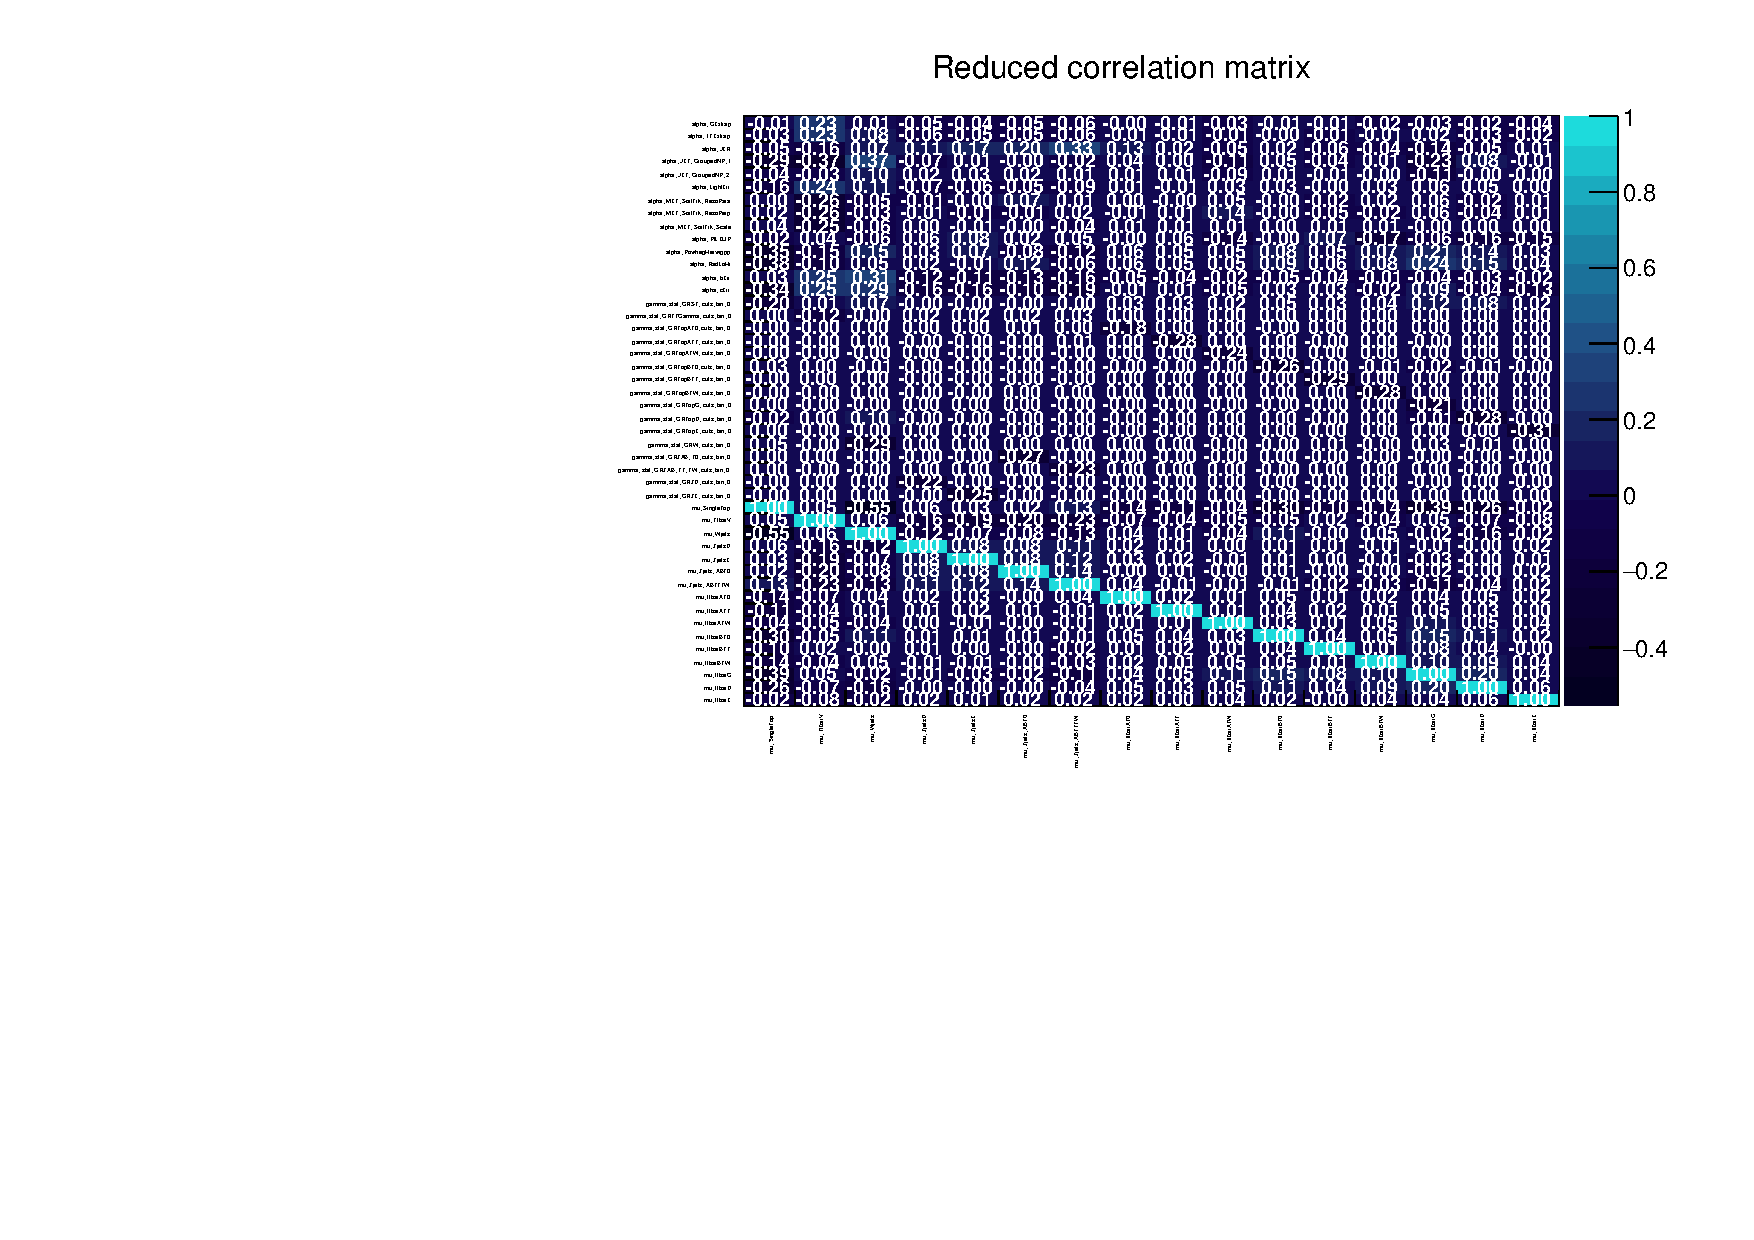
\includegraphics[width=\textwidth]{HistFitterStuff/corrMatrix.pdf}
		\caption{Correlation matrix between parameters of
      interest and nuisance parameters.}
		\label{figure.corrMatrix}
	\end{center}
\end{sidewaysfigure}

\clearpage
\begin{figure}[htbp]
	\begin{center}
		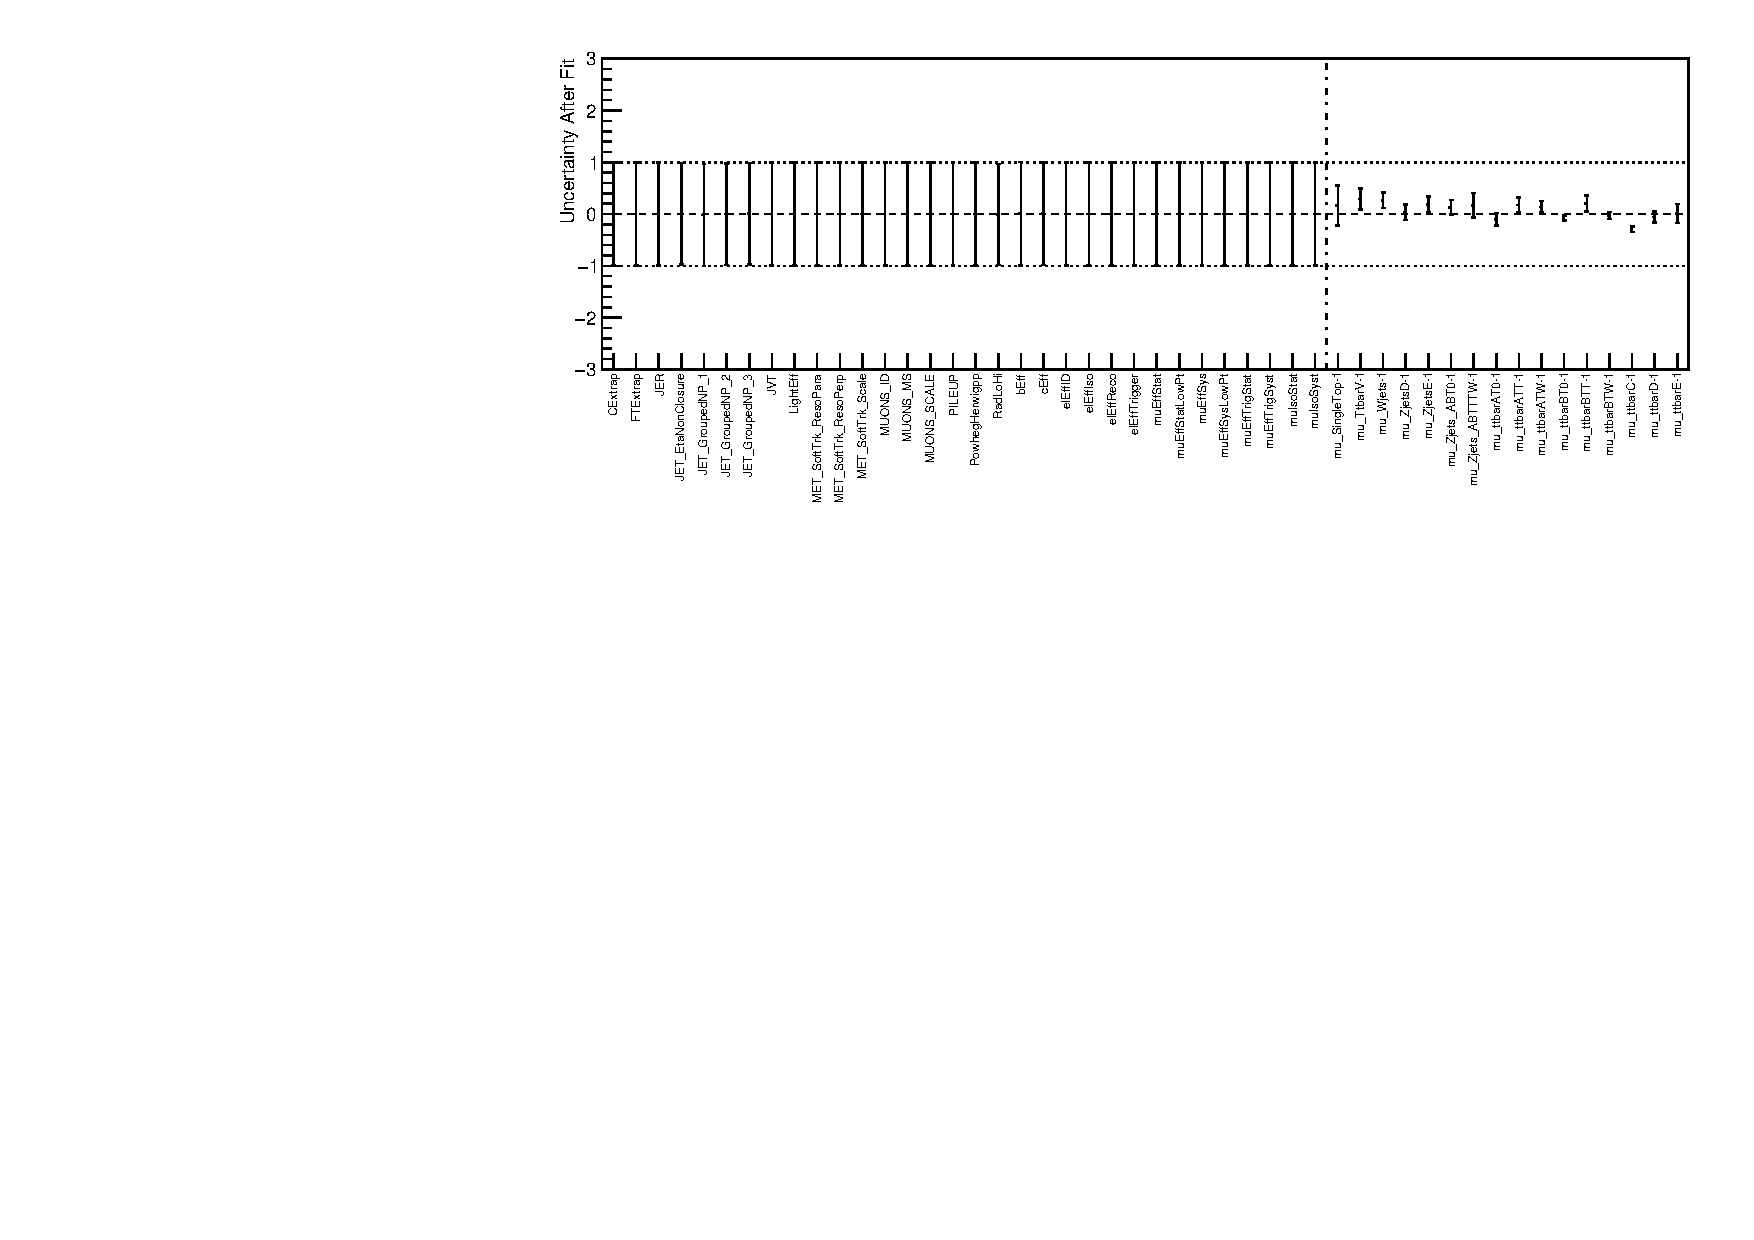
\includegraphics[width=0.85\textwidth]{HistFitterStuff/pullPlot.pdf}
		\caption{Post-fit pull plot for the background-only fit.}
		\label{figure.pullPlot}
	\end{center}
\end{figure}



\subsection{Exclusion-fit results}

\subsubsection{Results in the $m(\ninoone)$ vs $m(\stop)$ grid}

The results of the exclusion fit for SRA, SRB and SRC are shown in 
Figures \ref{figure.exclusion.SRA}, \ref{figure.exclusion.SRB} and
\ref{figure.exclusion.SRC} respectively. The signal regions are still
blinded so that the ``observed limit'' comes from setting the
observation equal to the background expectation from the Monte Carlo
(pre-fit).
The SRA (SRB) (SRC) results are
obtained by statistically combining the results from 
SRA\_TT, SRA\_TW and SRA\_T0 (SRB\_TT, SRB\_TW and SRB\_T0) (SRC1-5).
SRA, SRB and SRC are then combined by  taking the result with the best expected
$CL_s$; this combination is shown in Figure
\ref{figure.exclusion.SRABC}.

\begin{figure}[htbp]
	\begin{center}
		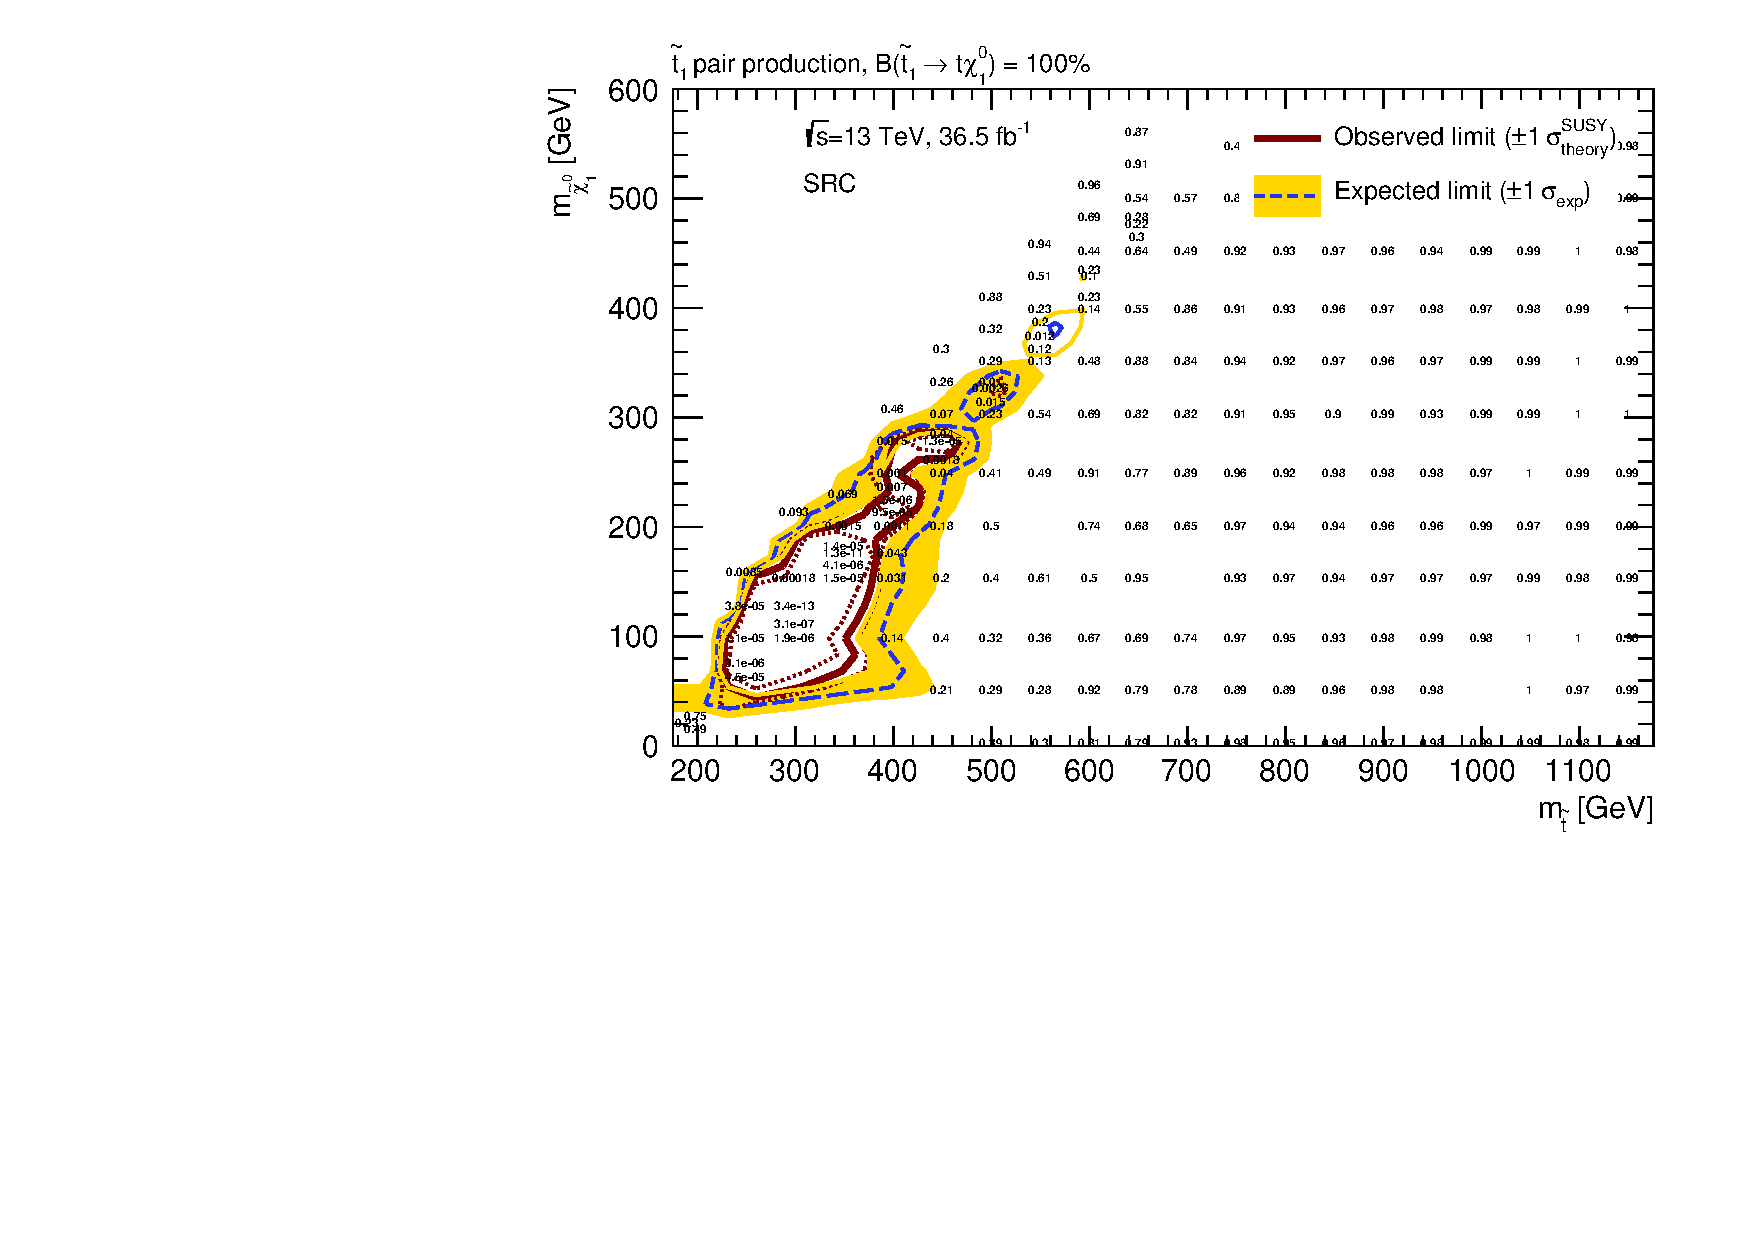
\includegraphics[width=0.85\textwidth]{HistFitterStuff/SRC_exclusion.pdf}
		\caption{Results of the exclusion fits in the tN1 grid from the
      combination of SRC1-5.  The numbers centered on the grid points
      indicate the expected CLs values.}
		\label{figure.exclusion.SRC}
	\end{center}
\end{figure}

\begin{figure}[htbp]
	\begin{center}
		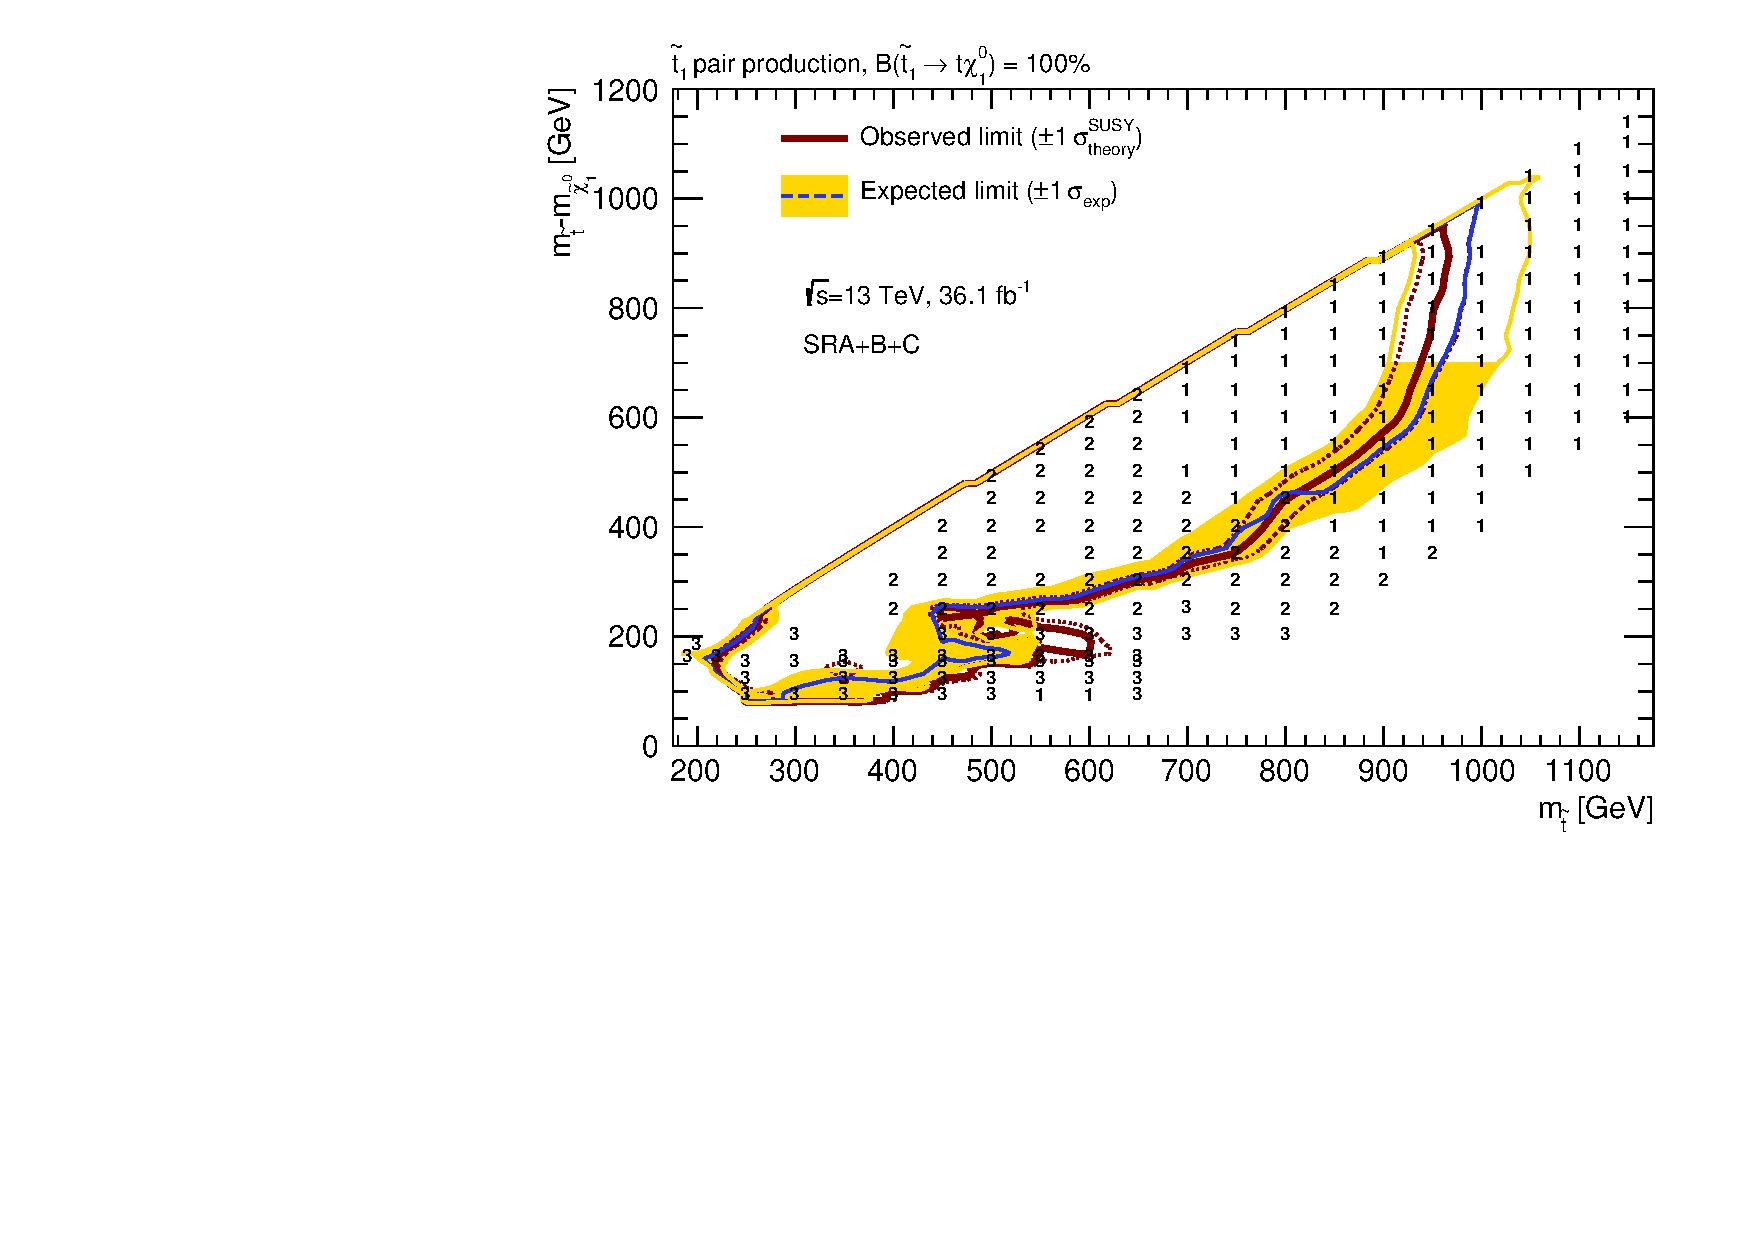
\includegraphics[width=0.85\textwidth]{HistFitterStuff/SRABC_exclusion.pdf}
		\caption{Results of the exclusion fits in the tN1 grid from the
      combination of SRA, SRB and SRC, based on the best
      expected $CL_s$. The numbers centered on the grid points
      indicate which of the signal regions gave the best
      expected $CL_s$ (with 1,2,3 corresponding to SRA,B,C
      respectively).}
		\label{figure.exclusion.SRABC}
	\end{center}
\end{figure}


